% Add `ngerman` to documentclass for German docs
\documentclass[12pt, a4paper]{article}
\usepackage{a4wide}
\usepackage{setspace}
\usepackage{csquotes}
\usepackage[utf8]{inputenc}

\usepackage{url}
\usepackage[hidelinks]{hyperref}
\usepackage{minted}
\usemintedstyle{perldoc}

% inline code
\newcommand{\code}[1]{\texttt{#1}}

% Uncomment for German
%\usepackage[ngerman]{babel}

% For generating template dummy text
\usepackage{lipsum}

\usepackage{myColors}
\usepackage{myFooter}
\usepackage{myTitle}

% Libraries outside of template
\usepackage[T1]{fontenc}
\usepackage{upquote}
\AtBeginDocument{%
    \def\PYZsq{\textquotesingle}%
}

\usepackage{amsmath}

\usepackage{verbatim}

%%%%%%%%%%%%%%%%%%%%%%%%%%%%%%%%%%%%%%%%%%%%%%%%%%%%%%%%%%%%%%%%%%%%%%%%%%%%%%%%

\project{CS 432 Web Science}
\author{Derek Goddeau}
\title{Assignment Eight}
\supervisor{Michael L. Nelson}

\doublespace
\pagestyle{hacker}

\begin{document}
\maketitle

\newpage



%%%%%%%%%%%%%%%%%%%%%%%%%%%
% Create Blog Term Matrix %
%%%%%%%%%%%%%%%%%%%%%%%%%%%
\section{Create a blog-term matrix}

To create the blog-term matrix I use the first $396$ lines of the \code{glutton.py} program. To get the 98 random blog URIs use the \code{requests} package with a ``next blog" request in a loop. Then I use \code{beautifulsoup} to parse out the RSS or Atom feed URIs out of the resulting page, and I save both to files so they do not need to be fetched again on new runs unless wanted.

To process each feed i use a while loop that iterates over all blog entries in the page and then attempts to get the next page, if an empty list is returned then the loop exits and returns the gathered data for the blog.

\begin{minipage}{\linewidth} % prevent splitting between pages
\vspace{2em}
\begin{minted}[fontfamily=tt]{python}
while entries:

    for entry in entries:
        .
        .
        .

    entries = []
    for link in feed_dict.feed.links:
        if link['rel'] == 'next':
        feed_dict = feedparser.parse(link['href'])
        entries = feed_dict.entries
\end{minted}
\vspace{2em}
\end{minipage}

\newpage
\noindent
While processing each entry \code{beautifulsoup} is used to get the words from each entry, the code is very similar to code from a previous assignment.

\begin{minipage}{\linewidth} % prevent splitting between pages
\vspace{2em}
\begin{minted}[fontfamily=tt]{python}
soup = bs(html, 'lxml')

[s.extract() for s in soup(
['style', 'script', '[document]'])]

text = (''.join(string.findAll(text=True))
        for string in soup.findAll())

words = [(word.strip()).lower()
         for string in text
         for word in string.split()
         if word.isalpha()]

# Remove any empty strings, just in case
words = list(filter(len, words))
\end{minted}
\vspace{2em}
\end{minipage}

The data is then pickled and saved so that this step too can be skipped on future runs if desired. But I also dump the data to plain text using code very similar to the PCI code as requested.

\newpage
\section{Create ASCII and JPEG dendograms}

The last \code{~200} lines of code in \code{glutton.py} were an attempt to use ``real" packages instead of the PCI to complete the rest. It uses \code{pandas} to read the pickled data into a data frame and then attempts to process the data using \code{scipy.cluster.hierarchy}. First I transform the data frame and then get the correlation between the rows, and then condense the matrix. Unfortunately I was unable to get it to work, after eating $\tfrac{3}{4}$ of my 32GB of RAM it throws \code{ValueError: Distance matrix 'X' diagonal must be zero}. Out of time I resorted to following essentially the directions from the slides.

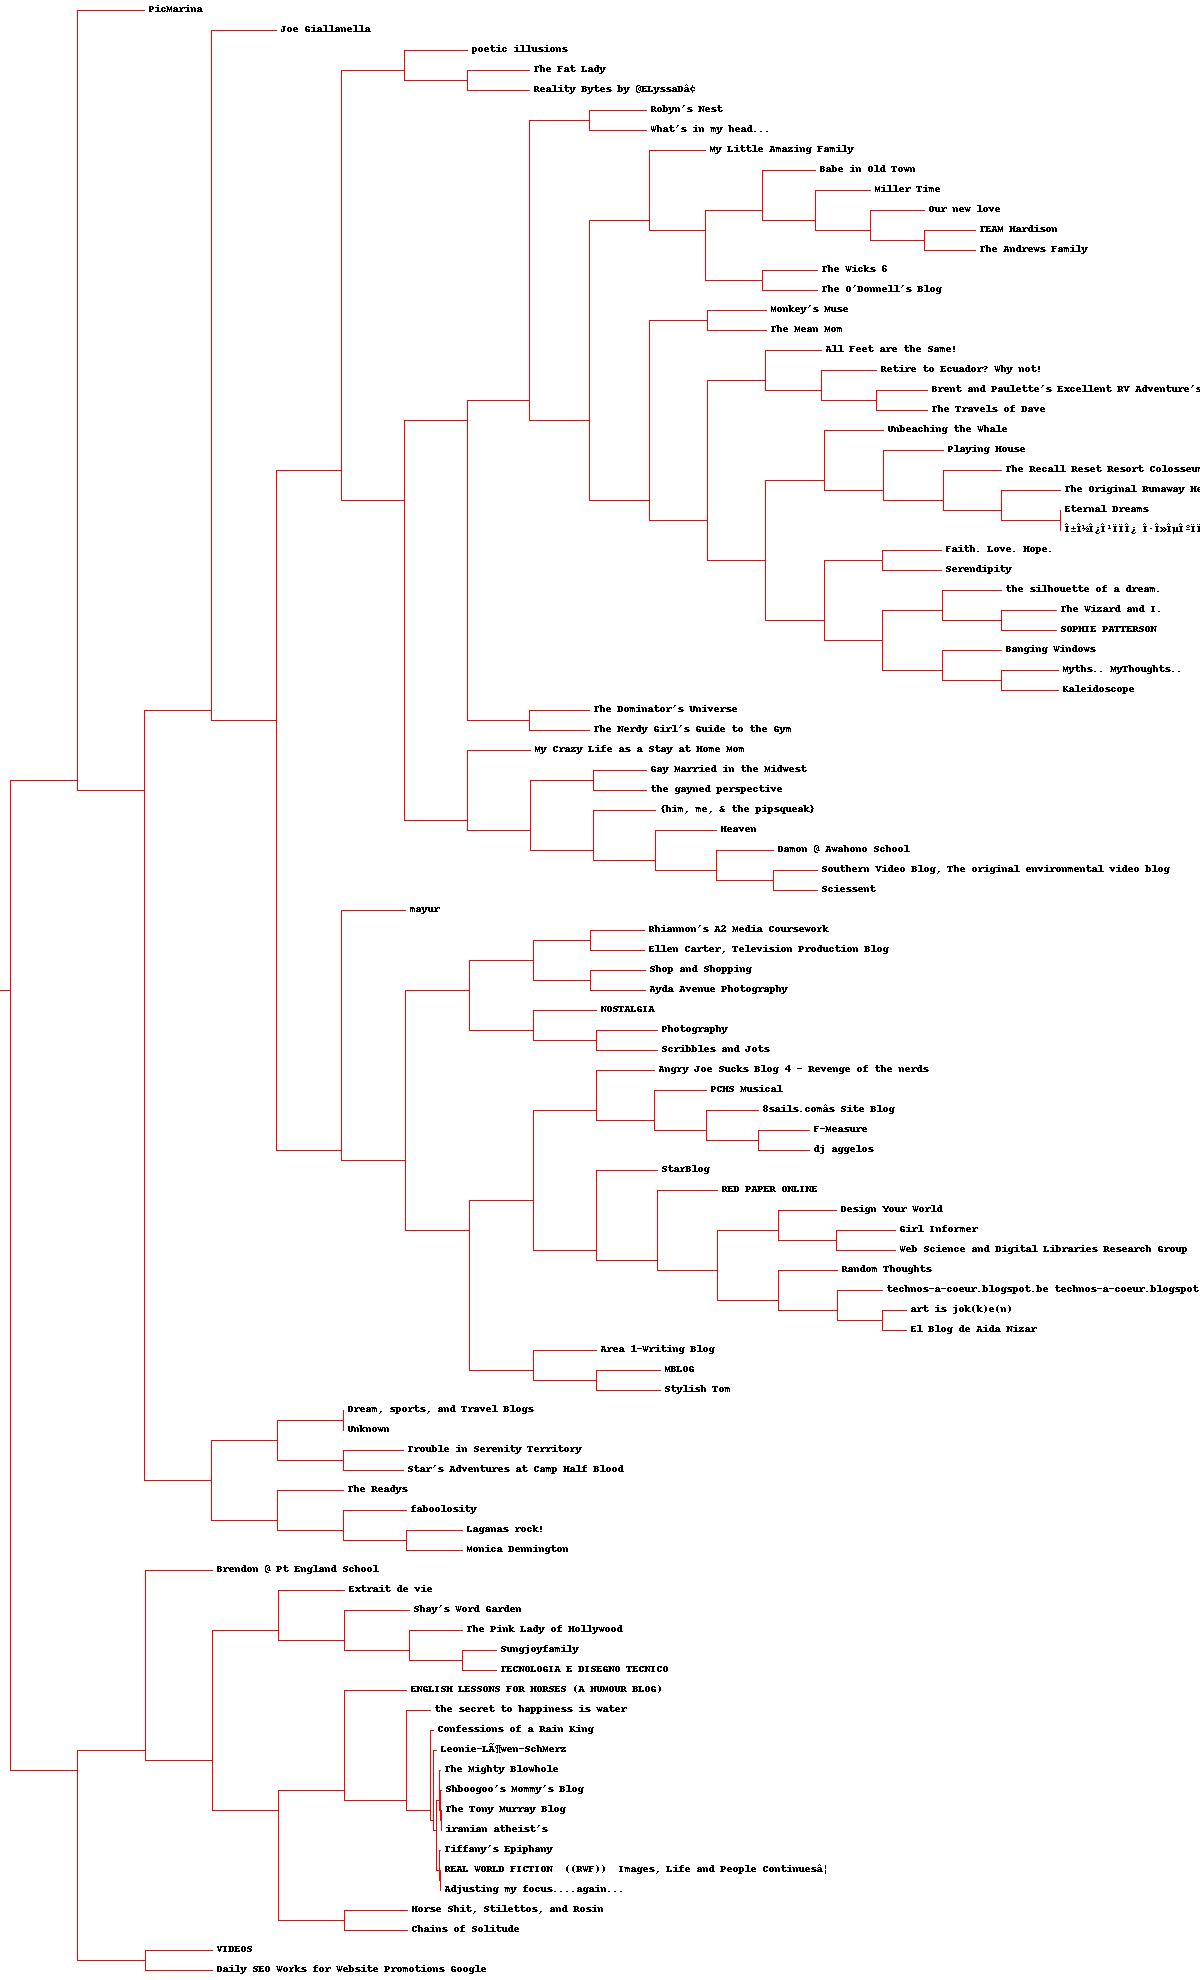
\includegraphics[width=\textwidth, height=\textheight]{../art/blogclust.jpg}

\section{Cluster the blogs using K-Means}

I really wanted to perform this using SciPy also but it just isn't working for me. With the PCI code I got the following.

\begin{table}[h]
\centering
\begin{tabular}{|c|c|}
\hline
\textbf{K} & \textbf{Iterations} \\ \hline
5          & 5                   \\ \hline
10         & 7                   \\ \hline
20         & 3                   \\ \hline
\end{tabular}
\end{table}

\newpage
\section{Use MDS to create a JPEG of the blogs}

It only ran for three iterations.

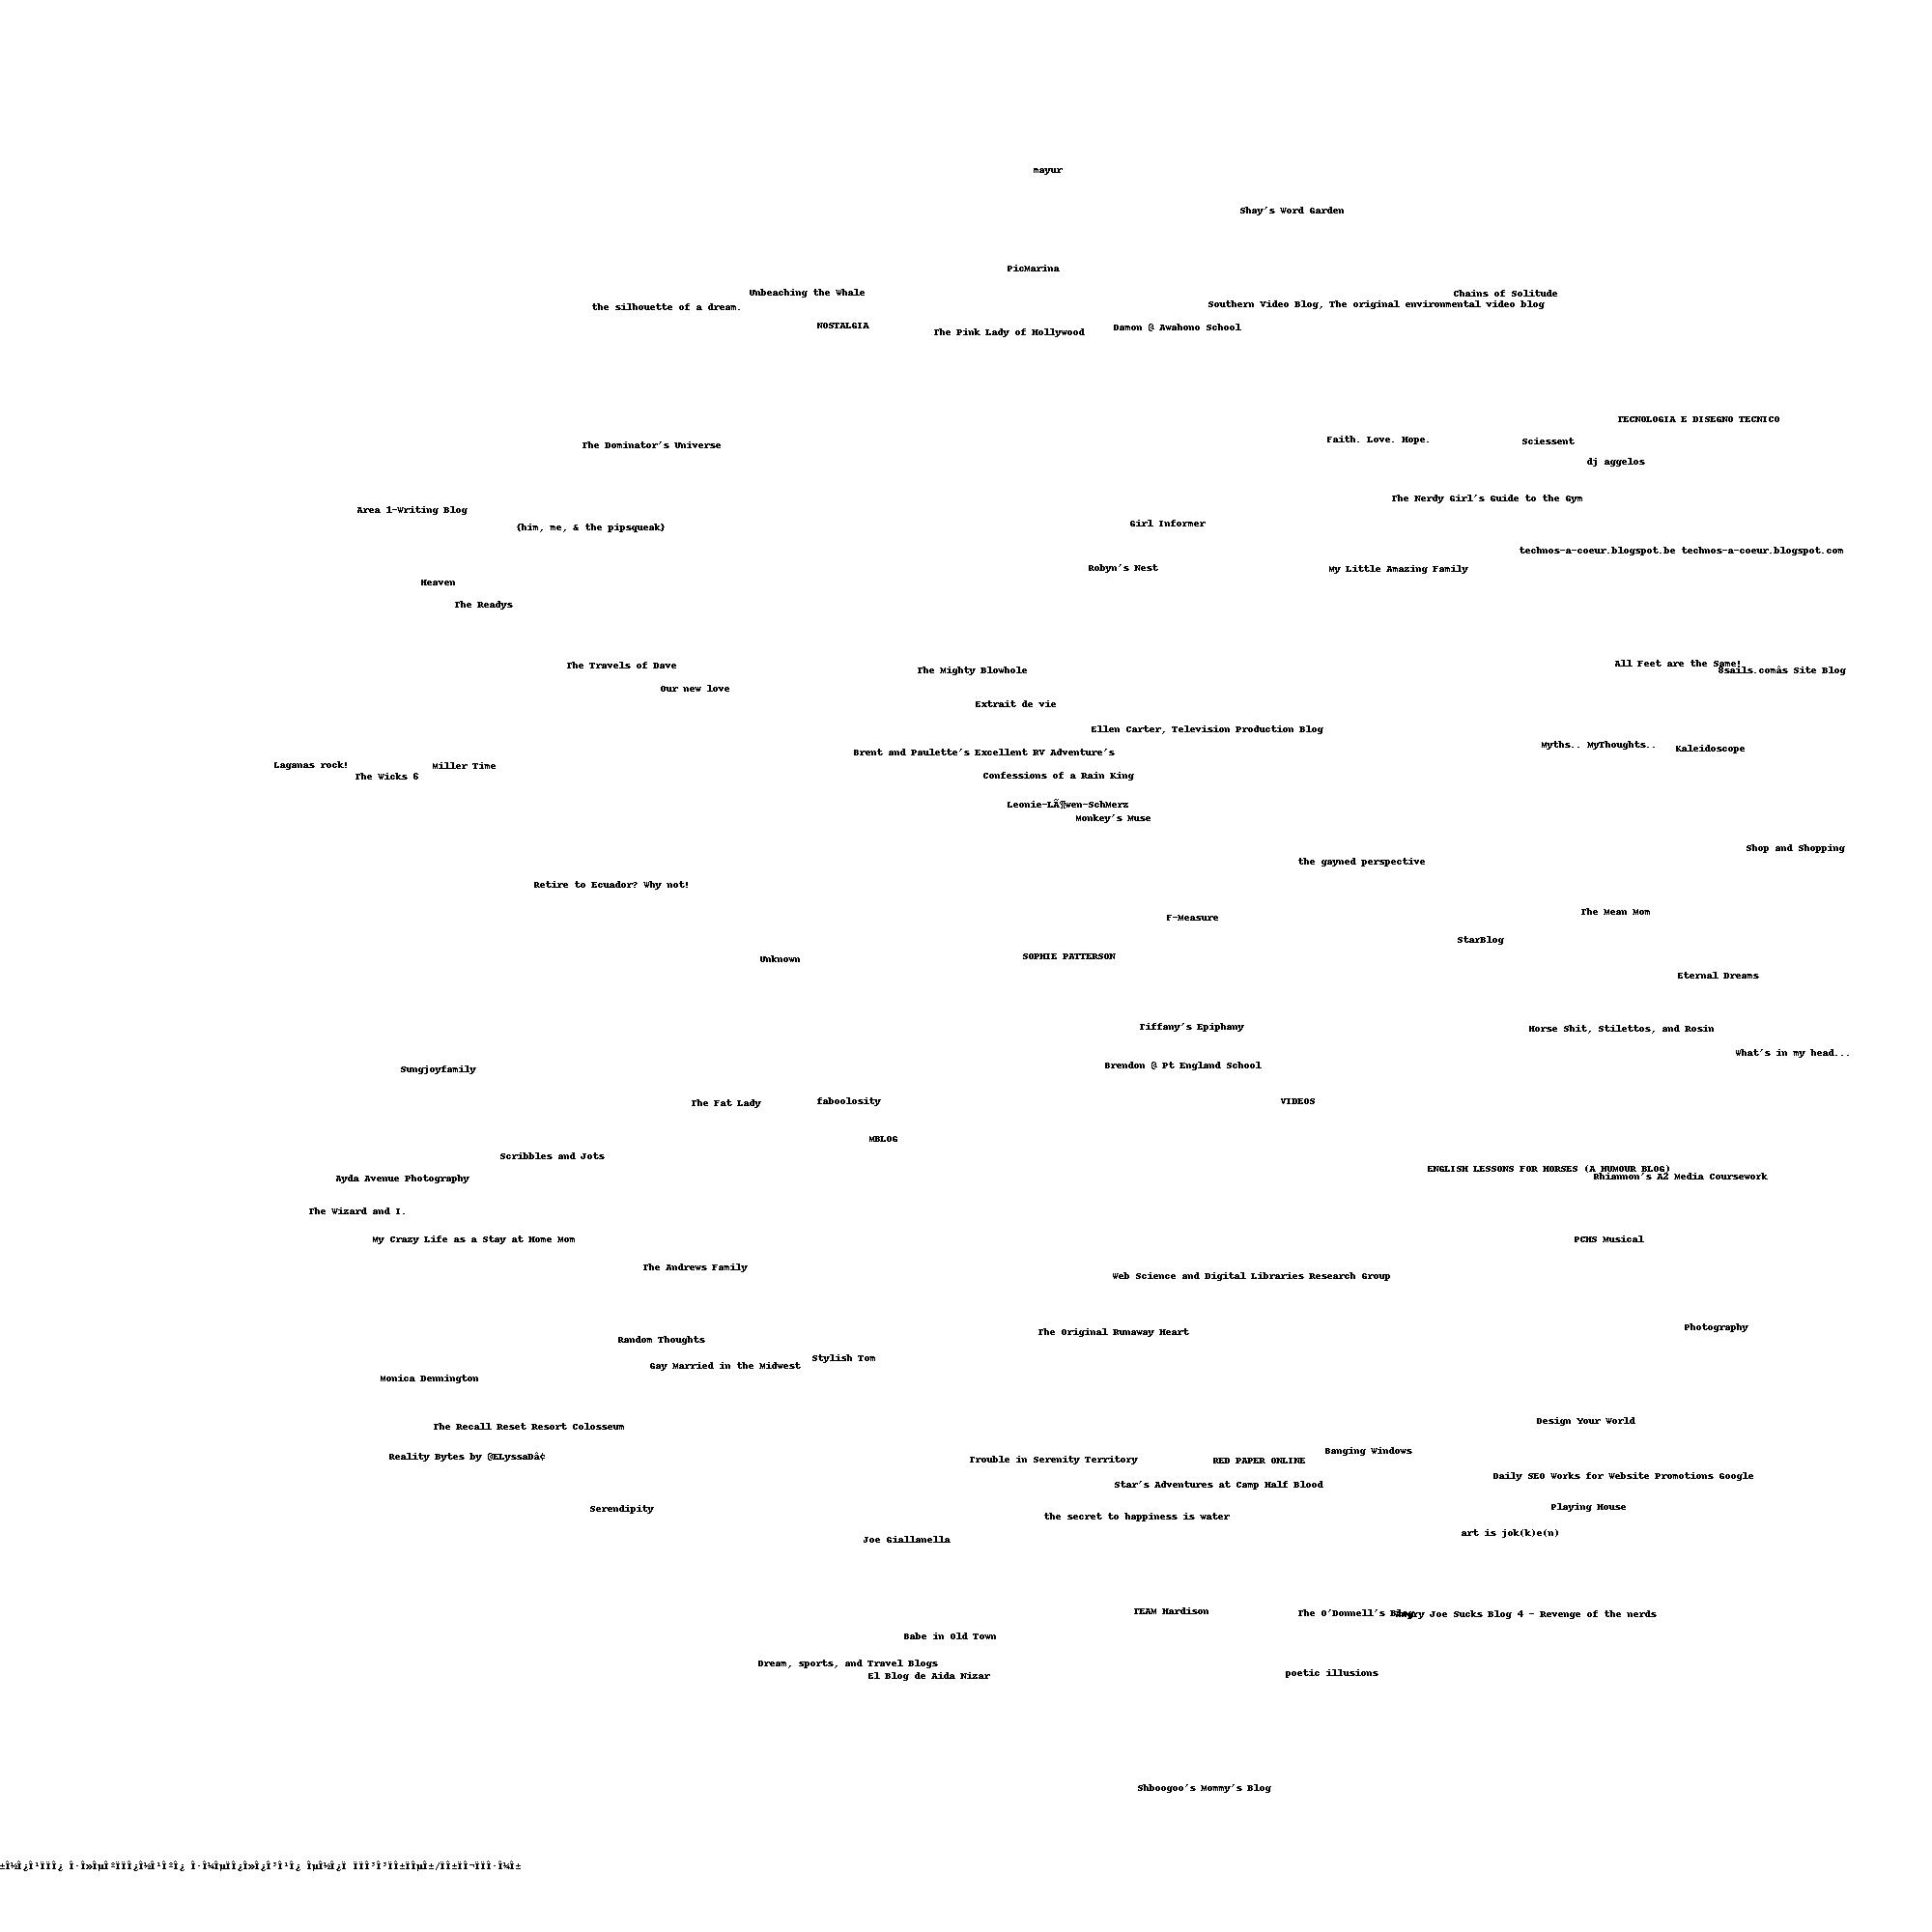
\includegraphics[width=\textwidth]{../art/blogs2d.jpg}

\newpage
\section{Blog URIs}

\verbatiminput{../data/uris.dat}


\end{document}
